\documentclass[10pt,a4paper]{article}
\usepackage[latin1]{inputenc}
\usepackage{amsmath}
\usepackage{amsfonts}
\usepackage{amssymb}
\usepackage{hyperref}
\usepackage{fullpage}

\usepackage{graphicx}% Include figure files
\usepackage{bm}% bold math
\usepackage{verbatim}
\usepackage{mathrsfs}
\usepackage{color}
\usepackage{paralist}
\usepackage{hyperref}
\usepackage{listings}

\title{ Exploring Weather trend }
%\date{}                                           % Activate to display a given date or no date

\begin{document}
\maketitle
\section{Introduction}
Global warming is a hot topic today.  On average, it is believed that Earth's climate system is warmer now than it was about eighty years ago. This implies that regions that are warm are getting warmer, while colder regions are becoming warm. Experts (including data scientists and analyst) see the trend is accelerating; they demonstrate global warming  by analyzing temperature data collected by weather stations on land and in the ocean, and by measurements of various effects of the warming.\\

\noindent This project provides a proof of global warming. Using the weather trend data on a database in Udacity portal, we have these objectives:
\begin{itemize}
\item  to analyze temperature trend in Victoria, the capital city of Canada province, British Columbia and compare with the global temperature trend, 
\item create a data visualization and finally,
\item write up our findings.
\end{itemize}
\section{Methodolody}
The computing languages used in this project include
\begin{enumerate}
\item SQL for extracting data from Udacity database 
\item  Pandas in Jupyter Notebook, for viewing and cleaning my data.
\item  Microsoft excel for calculations and creating chart.
\item LaTeX for writing this report.
\end{enumerate}

\subsection{Organizing the project}
The first thing to do is make sure that all our files relating to this project are organized in a single folder to ensure
efficient running of all codes. For example, to insert picture in this LaTeX file, we will need to have the picture stored in the same folder where the Latex file is. Hence since this project is for the Udacity Nanodegree program, I have a folder on my desktop called Udacity\_program, and in this folder I created another folder called Weather\_trend. This Weather\_trend will store all files concerning the weather trend project.
\subsection{Extracting data from Udacity database}
For this project, three tables in the database were provided with their corresponding instructions:
\begin{itemize}
\item city\_list - This contains a list of cities and countries in the database. Look through them in order to find the city nearest to you.
\item city\_data - This contains the average temperatures for each city by year (�C).
\item global\_data - This contains the average global temperatures by year (�C).
\end{itemize}
Therefore using the workspace connected to Udacity database schema, I wrote the following SQL queries to extract my data
\begin{enumerate}
\item  I live in Canada; so the following code will show me the list of cities in Canada from which temperature data was collected from.
\begin{lstlisting}
SELECT *
FROM city_list
WHERE country LIKE 'Canada'
\end{lstlisting}
Out of the six cities given, the city closest to where I live is Victoria, the capital city of the Canada province, British Columbia. 
\item  The following code extracts temperature data from Victoria city and join it with global data to obtain a single dataset.
\begin{lstlisting}
SELECT
        city_data.city AS "city_name",
        city_data.year AS "city_year", 
        city_data.avg_temp AS "city_average_temp.", 
        global_data.avg_temp AS "global_average_temp." 
    FROM 
        city_data 
    JOIN 
        global_data 
    ON 
        city_data.year = global_data.year 
    WHERE 
        city_data.city='Victoria' AND city_data.country='Canada'
        \end{lstlisting}

\end{enumerate}

%\begin{lstlisting}
%SELECT *
%FROM city_list
%WHERE country LIKE 'Canada'
%\end{lstlisting}
% \noindent \textit{Comment}: Using the following SQL query, I will now select Toronto's temperature data from city\_data \\[0.2cm]
% 
%\item Extracting data in Toronto city \textbf{city\_data}.
%\begin{lstlisting}
%SELECT year, avg_temp
%FROM city_data
%WHERE city = `Toronto' AND country = `Canada'
%\end{lstlisting}

\noindent Our final data has 186 rows and 4 columns. The column names include city\_name, city\_year, city\_average\_temp, and global\_average\_temp respectively. From the download link on the SQL database, I then export the result of this query to .csv.



\subsection{A look at the data/ data cleaning}
I opened up the downloaded csv file in Jupyter Notebook from my personal computer and performed the following operations:

\begin{itemize}
\item I wrote the following code to have a quick look at my data
\small
 \begin{lstlisting}[language=Python]
import pandas as pd                #importing pandas 

df=pd.read_csv('results-9.csv')    #we assign the csv file to the variable df
df.head()                          #prints few lines of my data

df.isnull().sum()                   #checks for missing values in data
\end{lstlisting}
\normalsize
\item  Result from the last command shows that there were three missing values in the Victoria temperature data. To fix the problem of missing data I wrote the following code:
\small
\begin{lstlisting}[language=Python]
#compute mean of Victoria temperature data and assign it to variable means
means = df['city_average_temp.'].mean()   

#fill missing values with (means) the calculated mean 
df['city_average_temp.'].fillna(means,inplace=True) 
\end{lstlisting}
\normalsize
which fills the missing values with the mean of the Victoria temperature data. 
\item I confirmed that the missing values were filled using the code
\small
\begin{lstlisting}[language=Python]
df.isnull().sum().any()
\end{lstlisting}
\normalsize
\item Finally I saved the changes to result\_edited.csv using the code
\small
\begin{lstlisting}[language=Python]
df.to_csv('result_edited.csv', index=False)
\end{lstlisting}
\normalsize
\end{itemize}

\section{Data Visualization}
I opened up the edited .csv file in Microsoft excel spreadsheet. 
\subsection{Creating chart for average temperature}\label{chart}
With the data opened on Microsoft spread sheet, I created a line chart with the following instruction
\begin{itemize}
\item from the table, highlight city\_year, city\_average\_temp and global\_average\_temp  columns respectively.
\item From Insert menu, choose the XY(Scatter) $>$ scatter with straight lines chart option and the chart is created.
\item Then from `Chart design $>$ Add Chart Element > Axis Titles, I labeled the horizontal and vertical axis respectively. Finally I gave the chart a title 
\item I saved chart as ave in .PDF format. This chart was appended into this .tex document using the following code
\end{itemize}

\begin{figure}[h!]
\begin{center}
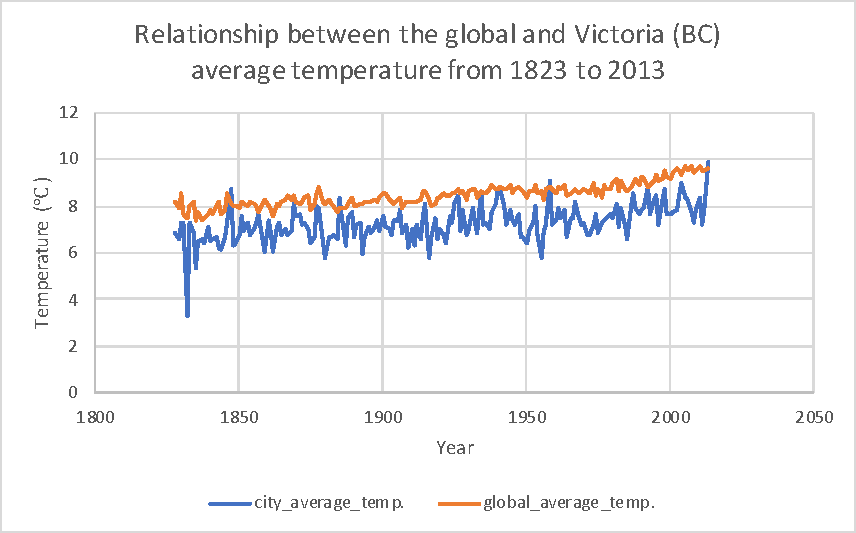
\includegraphics[width=0.75\textwidth]{ave}
\caption{ Comparing the global and Victoria (Canada) average temperature from the year 1823 to 2013. }
\label{setups}
\end{center}
\end{figure}
\small
\begin{lstlisting}
\begin{figure}[h!]
\begin{center}
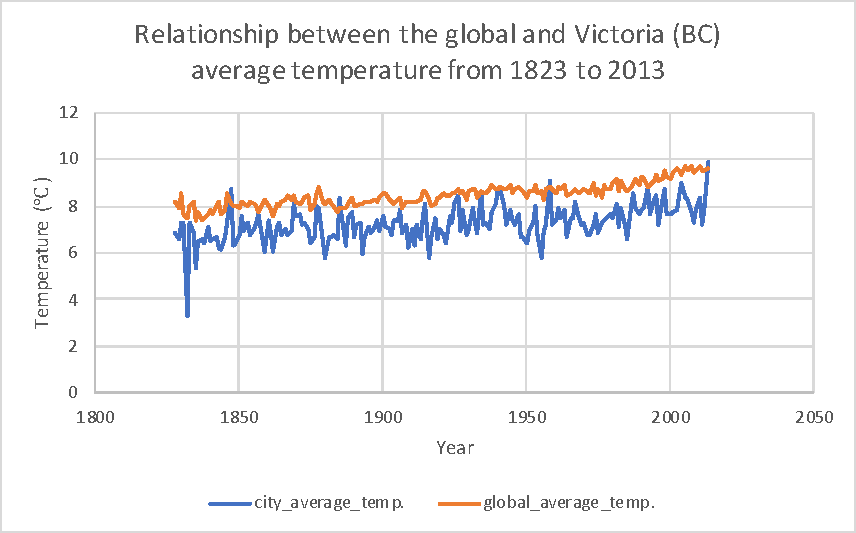
\includegraphics[width=0.75\textwidth]{ave}
\caption{ Comparing the global and Victoria (Canada) average temperature from 
the year 1823 to 2013. }
\label{setups}
\end{center}
\end{figure}
\end{lstlisting}
\normalsize

\noindent Fig \ref{setups} compares the temperature trend between Victoria city and the global temperature trend.  The fluctuations make it difficult to perform our analysis or give a proper report on the data set. A convenient tool is the moving average as we will see in the next section. 

\subsection{Moving averages}
Moving averages are used to smooth out data to make it easier to observe long term trends and not get lost in daily fluctuations. I calculated the 14-year moving average for each temperature data as follows
\begin{itemize}
\item I created two new columns, one titled 14-Day MA\_city where the 14-year moving averages for Victoria city would be stored, and the other titled 14-Day MA\_global, where the global moving average would be stored.
\item From the 14-Day MA\_city column, I scrolled down to the fourteenth (14) year (which is 1841) and used the AVERAGE() function to calculate the average temperature for the first fourteen years of temperature data (from 1823 - 1841). Then I dragged the cell all the way down to 2013 to fill the entire column with the formula. I repeated this process for the 14-Day MA\_global column.
\end{itemize}
\subsection{Creating chart for the moving averages}
Following the same procedure as in \ref{chart}, this time around with the city\_year, 14-Day MA\_city and 14-Day MA\_global columns respectively highlighted, the following chart was created
\begin{figure}[h!]
\begin{center}
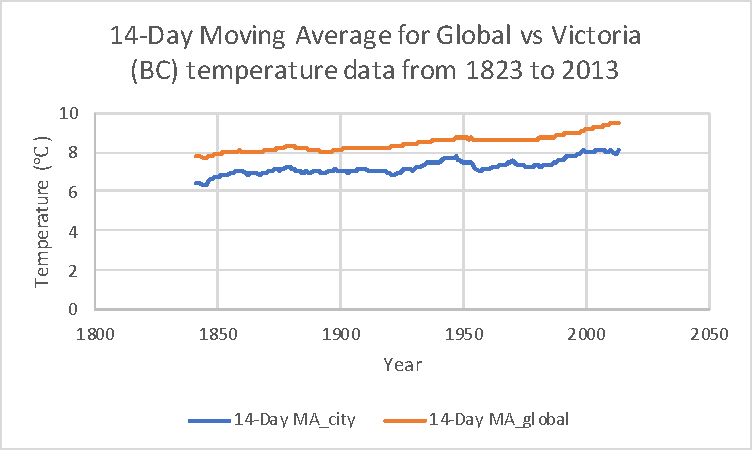
\includegraphics[width=0.75\textwidth]{temps}
\caption{ Comparing the 14-day moving average for global and Victoria (Canada) temperature trends. See inset for colour scheme}
\label{setup}
\end{center}
\end{figure}


\section{Observation}
\begin{itemize}
\item The positive increase in the line chart (Figure \ref{setup} ) between the global average temperature and the Victoria city over years, is indeed an indication that the world's climate is gradually warming up.
\item Figure \ref{setup} shows that the Earth was 1.74 degrees hotter in 2013 than it was in 1823, while Victoria city was 1.65 hotter in 2013 than it was in 1823. 
\item Canada is cold compared to many countries in the world and it is believed that its average temperature have warmed up by approximately 1.3 degrees which is about twice the global rate \cite{}. Our data and chart shows that average temperature warming in Victoria city still fall below the global average temperature. We can also observe from the chart that the last and most recent 13 years (2000-2013),  temperature across Victoria was steady with slight increase (about 0.06 degrees) across years, while the global average temperature continues to rise by 0.4 degrees. 
\item We can also observe from the chart that around the years (1887 -1922), temperature across Victoria and the Earth was steady with slight increase across years. 
\item The coldest year in Victoria and the Earth were observed in 1845 and 1844 respectively while the hottest years were 2005 and 2013 for Victoria city and the Earth respectively.
\end{itemize}
\end{document}  